\documentclass[conference]{IEEEtran}
\IEEEoverridecommandlockouts
% The preceding line is only needed to identify funding in the first footnote. If that is unneeded, please comment it out.

\usepackage{cite}
\usepackage{amsmath,amssymb,amsfonts}
\usepackage{algorithmic}
\usepackage{graphicx}
\usepackage{textcomp}
\usepackage{xcolor}
\usepackage{tikz}
\usetikzlibrary{arrows,shapes,positioning,shadows,trees,calc,intersections}

\newcommand{\boldvec}[1]{\boldsymbol{#1}}
\newcommand{\todo}[1]{\textbf{\textsc{{TODO: #1}}}}
\newcommand{\ico}[1]{\mathbf{#1}}
\newcommand{\sco}[1]{\uppercase{\mathbf{#1}}}
\newcommand{\vcr}[1]{#1}
\DeclareMathOperator*{\argmin}{\arg\!\min}
\DeclareMathOperator*{\argmax}{\arg\!\max}

\def\BibTeX{{\rm B\kern-.05em{\sc i\kern-.025em b}\kern-.08em
    T\kern-.1667em\lower.7ex\hbox{E}\kern-.125emX}}
\begin{document}

\title{A Virtual Reality Multi-Sensor 3d Reconstruction System}

\author{\IEEEauthorblockN{ Markus Friedrich, Kyrill Schmid}
\IEEEauthorblockA{
\textit{Ludwig-Maximilians-University Munich}\\
Munich, Germany \\
\{markus.friedrich / kyrill.schmid\}@ifi.lmu.de}
}

\maketitle

\begin{abstract}
We propose the concept for a distributed multi-sensor 3d reconstruction system that includes a virtual reality (VR) scan visualization component. It fuses depth data from two different sources: A mobile time-of-flight (ToF) depth sensor and an image-based 3d reconstruction module that estimates depth based on camera images.
The continuously evolving 3d data set is visualized on-the-fly in a specialized VR application which allows for interactive scanning scenarios.
Currently, two sensors are considered but we plan to extend the system to support a multitude of depth sensors that iteratively contribute to the global data set.  
\end{abstract}

\begin{IEEEkeywords}
depth sensor fusion, distributed 3d reconstruction, virtual reality, data visualization
\end{IEEEkeywords}

\section{Introduction}
The advent of cheap depth sensors shipped in consumer devices like the Microsoft\textsuperscript{\textcopyright} Kinect\texttrademark \space or the Asus\textsuperscript{\textcopyright} Zenfone AR\texttrademark \space has led to a boost in 3d reconstruction research (see e.g. \cite{Graber2011,Steinbruecker13,fuhrmann2011}) and 3d scanning application development. 
At the same time, virtual reality (VR) hardware has left the labs and is now mature enough for widespread adoption.    
\\
In this work, we introduce a concept that combines the best of both worlds through a distributed multi-sensor 3d scanning system that allows a user to scan real-world objects while providing instantaneous feedback on the quality and shape of the already measured object parts using a VR-based visualization.
\\
The system uses a Zenfone AR\texttrademark \space device which is equipped with a time-of-flight (ToF) sensor as main source for depth values. 
Since the used VR head-mounted display (HMD) comes with a front-facing camera, we would like to use it to compute additional depth values in complement to those provided by the Zenfone AR\texttrademark \space using an image-based 3d reconstruction approach\cite{Seitz2006}. 
We exploit the fact that for each image, the pose of the camera is known since it is fixed on the HMD and the HMD computes its exact pose which is needed for VR applications.
In addition, the internal camera parameters (e.g. focal length and pixel resolution) are well-known and do not change over time.   
\\
Our system consists of the following core components:
\begin{itemize}
\item A 3d reconstruction component that estimates depth values based on images that come from the front-facing camera within seconds ($\leq 2\text{s}$) for each incoming image. 
\item A depth value fusion strategy that merges depth values from different sources into a single consistent data set in near real-time (maximum delay $\leq 2\text{s}$).
\item A VR visualization module that is able to blend depth measurements into the camera image of the real-world object without artefacts and noticable delays in order to avoid VR sickness symptoms. 
\end{itemize}
Currently, the system uses two depth sensors. 
Next steps involve the support of a multitude of depth sensors that all contribute to the global data set.   
\section{Background}

%\subsection {Affine Spaces and Transformations}
%3d data is described using the 3d real Euclidean point space $\mathcal{E}$. 
%It can distinguish between points and vectors and is formulated as a real affine space $\mathcal{A}$.
%$\mathcal{A}$ consists of a real point space $S$ and a real Euclidean vector space $V$ with an orthonormal basis $v_1,v_2,v_3$.
%Together with the origin $\sco{o}\in S$, the basis $v_1,v_2,v_3$ forms the affine system $(\sco{o};v_1, v_2, v_3)$.
%It can be used to express a point $\sco{p}\in S$ uniquely as
%$$ \sco{p} = \sco{o} + x_1\vcr{v_1}+x_1\vcr{v_2}+x_3\vcr{v_3},$$
%where $x_i \in \mathbb{R}^3$.
%The $n-$tuple $(x_1,\ldots,x_n)^T \in \mathbb{R}^3$ is called affine coordinates and is also a unique description of a point $\sco{p}\in S$.\\
%Important point transformations comprise translation, rotation and scaling.
%These are affine transformations $f:U \to V$ between two affine spaces $U$ and $V$, and can be written as 
%\begin{equation} \label{eq:afftrans}
%\sco{p} \mapsto M \sco{p} + \vcr{t},
%\end{equation}
%where $M$ is a linear transformation expressed as an $3\times 3$ matrix, $\vcr{t}$ is a translation vector and $\sco{p}\in U$. 
\subsection {Rigid Body Poses}
The 3d pose (position and orientation) of a rigid body (e.g. a camera) can be described by $4\times 4$ matrices of the form 
$$ 
T = 
\left(
\begin{array}{c|c}
	R & \vcr{t} \\ \hline
	0_{1\times 3} & 1 \\
\end{array}
\right),
$$
where $t\in \mathbb{R}^3$ is the translation vector and $R$ is a $3\times 3$ rotation matrix.
$R$ is orthogonal and has a determinant of $+1$.
$T$ represents a rigid body pose and has thus six degrees of freedom (three for translation and three for rotation).  
The matrix $T_{AB}$ represents the coordinate frame transformation from frame $B$ to frame $A$.
\subsection {Voxels \& Truncated Signed Distance Functions}
Voxels can be seen as 3d pixels that discretize a certain subset of the 3d real Euclidean point space. 
Each voxel stores a domain-specific $n$-tuple (e.g. signed surface distance and color).
When stored in a regular grid, space complexity is $\mathcal{O}(n^3)$. 
More space efficient data structures exist, e.g. hierarchical space partitioning schemes or spatial hash maps \cite{Niessner2013}. 
\\
A signed distance function $d: \mathbb{R}^3 \mapsto \mathbb{R}$ maps a point $\sco{x}$ to a signed value that represents the distance between the point and the surface of an object. 
Thus, the surface is implicitly defined by the zero-set of $d$: $\{\sco{x} \in \mathbb{R}^3 : d(\sco{x})=0\}$.
\\
Truncated signed distance functions (TSDFs) are only defined for a certain distance interval and are - in their discretized form - widely used for depth sensor fusion (e.g. in \cite{Graber2011}).
Our system uses a voxel-based surface representation in combination with discretized TSDFs, where each voxel stores a TSDF value, a color and a fusion weight.    

\subsection {3d Reconstruction}
The goal of 3d reconstruction is to estimate the surface of real-world objects based on sensor data. 
Our system currently foresees two different depth value sources: 
A ToF sensor that measures the phase shift between an emitted and the corresponding reflected infrared light pulse in order to estimate the distance to an object. 
And a method that estimates depth using techniques from stereophotogrammetry that work on calibrated camera images \cite{Seitz2006}. 
The term calibrated means that for each image, the corresponding pose $T_{WC}$ of the camera is known and can be used to transform a point from the camera coordinate frame to the world coordinate frame.

\section{Related Work}
Real-time 3d reconstruction, depth value fusion and voxel visualization in real-time is a well-established field of research \cite{Graber2011,Steinbruecker13,fuhrmann2011}. 
One example is the work of Graber et al. \cite{Graber2011} that uses similar methods for 3d reconstruction and fusion than we do. 
The main difference to our work is the missing VR approach for visualization. 
A combination of 3d scanning and VR is proposed in \cite{danhof2015}. 
The authors describe a VR-based, user-guided 3d scanning simulator that uses the VR controller as a virtual depth sensor. 
Created point clouds are visualized within the VR application.
While related to our system, it does not deal with real data. 
\section {Concept}
The current system design foresees four hardware components: A workstation for sensor fusion and data set visualization (1), a workstation for 3d reconstruction based on camera images (2), a VR controller with mounted depth sensor (3, Asus\textsuperscript{\textcopyright} Zenfone AR\texttrademark \space) and the VR HMD (4, HTC\textsuperscript{\textcopyright}  Vive\texttrademark \space) as display and camera.  
\\
The depth sensor is attached to the wireless VR controller in order to get its pose in the VR system's coordinate frame (up to a fixed offset). 
This is necessary in order to transform incoming depth values into the world coordinate frame for sensor fusion. 
The user holds this controller during the scan process and moves it around the object that should be scanned. 
\\
The HMD displays the scene which contains both, the current camera image and the rendered global data set containing the already scanned object parts. 
Without showing the latest camera image, the user would lose orientation during the scan process.
See Figure \ref{fig:system} for an overview of the system.
\begin{figure}[!htbp]
	\centerline{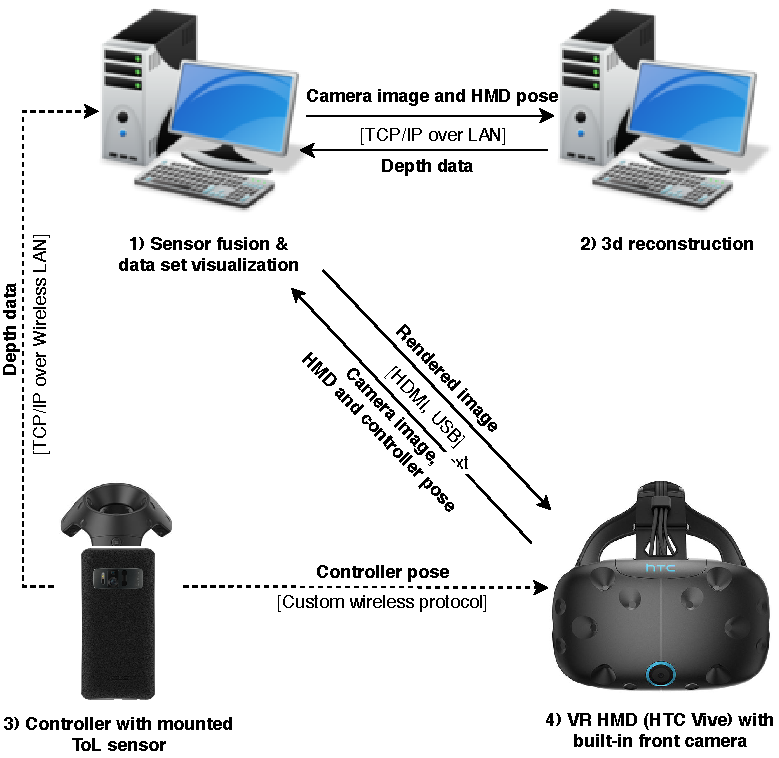
\includegraphics[width=0.45\textwidth]{figures/3dsystemoverview.pdf}}
	\caption{Overall system architecture. Communication protocols are denoted in square brackets. Note that the selected VR system also uses two additional sensor boxes for HMD pose estimation. Since their role is transparent, they are ommitted in this diagram. }
	\label{fig:system}
\end{figure}

\subsection {3d Reconstruction}
\label{ch:3drec}
The 3d reconstruction component (Figure \ref{fig:system}, component 2) uses a variant of the plane-sweep method to retrieve depth values from a series of calibrated images recorded by the front-facing camera \cite{Collins96}. 
It is optimized for modern GPUs and achieves near real-time performance on images with HD resolution.
\\
Its principles are derived from basic triangulation. 
Corresponding image points are searched with help of pixel color-based similarity measures within calibrated views.
With known correspondences in at least two views, the scene point can be estimated.
\\
The detailed explanation of the method is based on Figure \ref{fig:planesweep}.
\begin{figure}[!htbp]
	\centering
	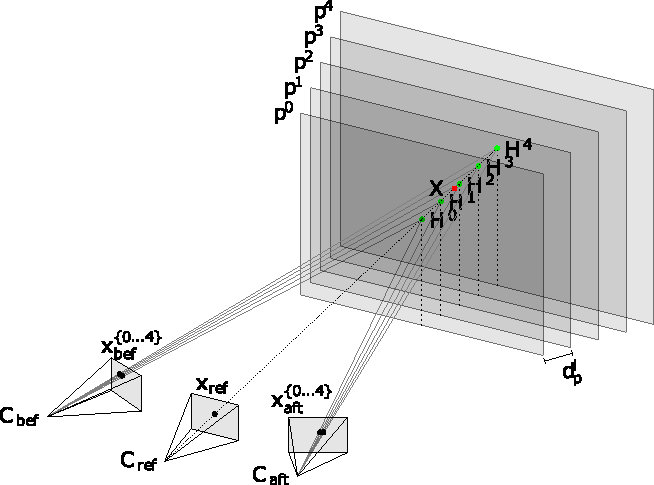
\includegraphics[width=0.40\textwidth]{figures/planesweep}
	\caption{
		The plane-sweep setting for a reference view, two sensor views and constant plane distances $d_p^i$.}\label{fig:planesweep}
\end{figure}
A reference camera view and two other camera views with centers $\sco{C}_{\text{ref}}$,$\sco{C}_{\text{bef}}$ and $\sco{C}_{\text{aft}}$ with partially overlapping frustums are considered.
\\
The scene point $\sco{x}$ (red point) corresponding to an image point $\ico{x}_{\text{ref}}$ (black point) in the reference view is to be estimated.
$\sco{x}$ has to be located on the view ray $v_{\text{ref}}$ through the camera center $\sco{C}_{\text{ref}}$ and the image point $\ico{x}_{\text{ref}}$.
\\
In order to estimate $\sco{x}$, a set of $n_p$ so-called sweeping planes $\{p^0,\ldots,p^{n_p-1}\}$ parallel to the view plane of the reference camera are placed along $v_{\text{ref}}$.
They divide the reconstruction volume.
The distances between the sweeping planes, $d_p^i, i\in\{0,\ldots,n_p-1\}$, can be user-defined and constant or determined by more sophisticated methods. 
\\
The intersection points between sweeping planes and view ray $v_{\text{ref}}$, $\sco{h}^i$ (green points), are estimates of the location of $\sco{X}$.
In order to determine the best candidate $\sco{H}^b$, all $\sco{h}^i$ are consecutively projected on the view planes of the views $V_{\text{bef}}$ and $V_{\text{aft}}$, resulting in image points $\ico{x}_{\text{bef}}^i$ and $\ico{x}_{\text{aft}}^i$ (black points).
Correlation measures $c_{\text{bef}}^i, c_{\text{aft}}^i \in [0,1]$ are then computed based on the color values of the view images $I_{\text{ref}}$ and $I_{\text{bef}}$ at $\ico{x}_{\text{ref}}^i$ and $\ico{x}_{\text{bef}}^i$ (resp.\ $I_{\text{ref}}$ and $I_{\text{aft}}$ at $\ico{x}_{\text{ref}}$ and $\ico{x}_{\text{aft}}$).
Suitable correlation measures are e.g. the Euclidean distance or normalized cross-correlation \cite{Lewis1995}.
The best candidate index $b$ is then determined by 
$$b = \argmax_{i\in\{0,\ldots,n_p-1\}}{(\max(c_{\text{bef}}^i,c_{\text{aft}}^i))}.$$
Thus, the sweeping plane with the best overall correlation value is chosen. 
The plane-sweep method is parallelizable (one thread per image point in the reference view) and can therefore be executed efficiently on GPUs
In addition, the quality is adjustable by changing the sweeping plane distances $d_p^i$ which alters the number of sweeping planes $n_p$.
\subsection {Depth Sensor Fusion}
\label{ch:fusion}
All scene points estimated during a 3d reconstruction iteration and all new scene points from the ToF sensor need to be integrated into the global data set (Note that the ToF sensor automatically converts a scalar depth value to a full 3d scene point and all scene points are relative to the coordinate frame of their corresponding camera or sensor). 
This is done by the fusion component (Figure \ref{fig:system}, component 1).
\\
For fusion, a simple and well-known voxel fusion approach was selected \cite{Curless1996}.
For each voxel, the estimated signed distance $D$ to the real surface is stored together with a fusion weight $W$ which serves as a confidence measure.   
\\
Each scene point is transformed from camera-space to world-space using $T_{WC}$, resulting in the world-space scene point set $\{s_i\}$. 
The estimated distance to the surface, is defined for a certain interval $t_{max}$ along the scene point's view ray $v_i$ (with a distance of $0$ at the exact position of the scene point).
This represents the TSDF $d_i(\cdot)$ for that particular scene point defined on its view ray, see Figure \ref{fig:tsdfcreation} for an example. 
\\
The view ray interval in world-space is then discretized based on the edge length of a voxel $e_v$. 
For each sample point $\sco{x}$, $d_i(\cdot)$ is evaluated.
The set of resulting signed distances is then fused with the voxels in the grid at $\sco{x}$. 
The new distance value $D^{*}$ at grid position $\sco{x}$ is computed by
\begin{equation}
\label{eq:levoy1}
D^{*}(\sco{x}) = \frac{W(\sco{x})D(\sco{x})+w_{i}d_{i}(\sco{x})}{W(\sco{x})+w_{i}},
\end{equation}
where $w_{i}$ equals the correlation value of the corresponding scene point.
The equation for calculating the new fusion weight $W^{*}$ is 
\begin{equation}
\label{eq:levoy2}
W^{*}(\sco{x}) = W(\sco{x}) + w_{i}.
\end{equation}
Figure \ref{fig:levoyfusion} shows an example of this fusion scheme.
\begin{figure}[!htbp]
	\centering
	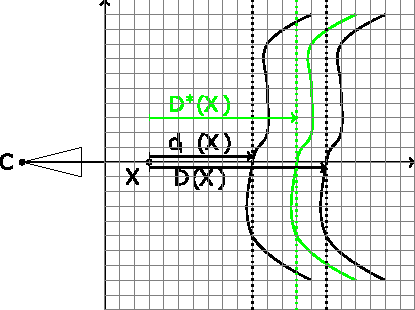
\includegraphics[width=0.35\textwidth]{figures/tsdf1}
	\caption{
		The signed distance to the surface, $D(\sco{x})$, at position $\sco{x}$ is updated by the signed distance, $d_{i}(\sco{x})$ at that position.
		The influence of both values is determined by the weights $W(\sco{x})$ and $w_{i}$.
		The new signed distance $D^{*}(\sco{x})$ is illustrated in green.
	}
	\label{fig:levoyfusion}
\end{figure}
\begin{figure}[!htbp]
	\centering
	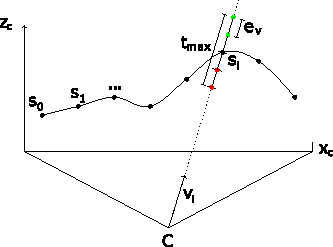
\includegraphics[width=0.30\textwidth]{figures/fusion1}
	\caption{
		Illustration of the TSDF value generation process reduced to the $xz$-plane in camera coordinates.
		Green dots indicate positive signed distances, red dots negative ones.     
	}
	\label{fig:tsdfcreation}
\end{figure}
\\
In \cite{Curless1996}, a grid in combination with run-length encoding (RLE) for data compression is employed as voxel storage data structure. 
A more elaborate data structure based on hash mapping principles was tested for the proposed system concept \cite{Niessner2013}. 
It stores small cubes of $8\times8\times8$ voxels in a spatial hash map with a hash function proposed by Teschner et al.\ \cite{Teschner2003}.
It reads 
$$h(x,y,z) = ((x a)\oplus(y b)\oplus(z c))\bmod n_b,$$
where $a = 86{,}028{,}157$, $b = 73{,}856{,}093$, $c = 19{,}349{,}663$ are large prime numbers, $n_b$ is the number of hash map buckets and $\oplus$ is the bitwise XOR operator. 
It is parametrized by the integer world-space position of the voxel cube $(x,y,z)^T$.



\subsection {Visualization}
\label{ch:vis}
The visualization of implicit surfaces stored in voxels can be done using sophisticated ray-tracers like the one employed in \cite{Graber2011b}. 
Another option would be to generate a polygon mesh with help of the marching cubes algorithm \cite{Lorensen1987} which is then rendered using standard 3d engines.
Sophisticated 3d point cloud renderers can be employed as well but then only voxels with a signed distance of $0$ can be considered in order to avoid cluttering.
\\
We have implemented a basic renderer that retrieves voxel cubes from the hash map and renders small camera aligned rectangles for each voxel. 
See Figure \ref{fig:renderpipe1} for details.
\begin{figure}[!htbp]
	\centering
	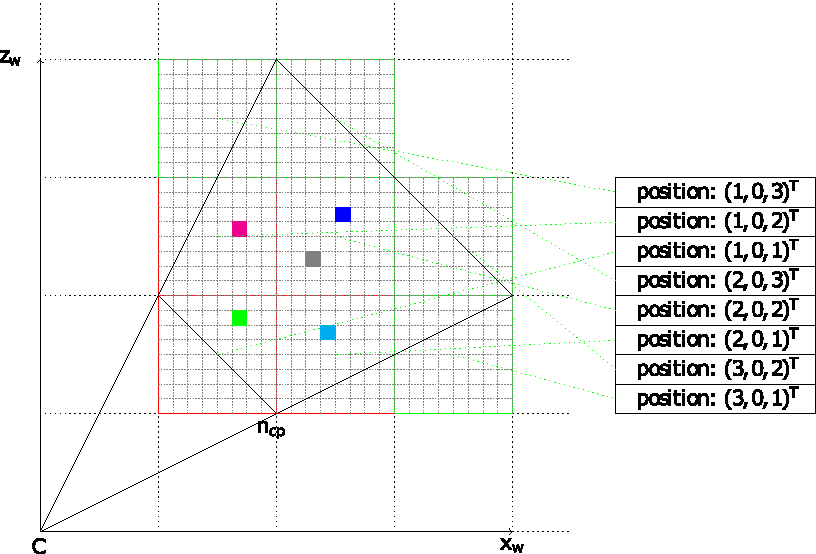
\includegraphics[width=0.40\textwidth]{figures/renderpipe1}
	\caption{
		The render pipeline.
		The scene camera frustum (black lines) is defined by the camera origin $\sco{C}$, the near clipping plane $n_{cp}$ and the far clipping plane $f_{cp}$ (its orientation is indicated by the orientation of the black triangle). 
		Eight potential voxel cubes (green and red lines) lie within or intersect with the frustum. 
		Their positions are saved in the query voxel cube position list which is used to query for voxel cubes within the frustum.  
		Note that only those voxel cubes surrounded by red lines are existent in the fusion data structure.  
	}
	\label{fig:renderpipe1}
\end{figure} 
Figure \ref{fig:rendering} shows a low-res voxel visualization with ca. $20,000$ voxels.
\begin{figure}[!htbp]
	\centering
	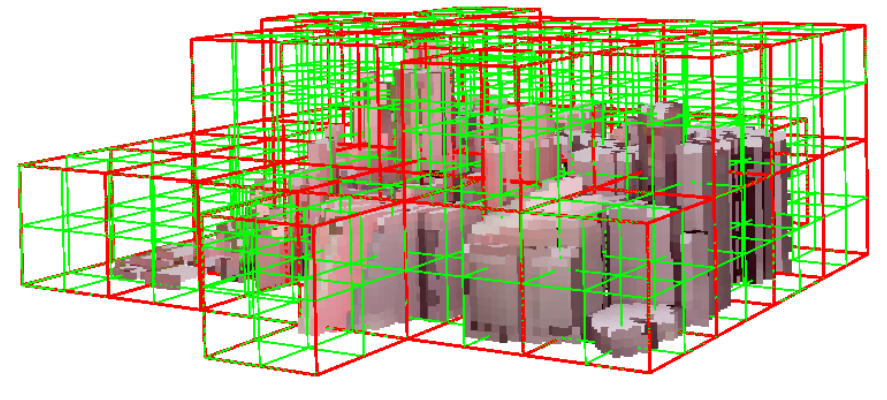
\includegraphics[width=0.45\textwidth]{figures/rendering.png}
	\caption{
		Voxel set test rendering with around $20,000$ voxels. The green boxes indicate voxel cubes. 
	}
	\label{fig:rendering}
\end{figure} 

\section {Status Quo, Questions and Future Work}
In context of this project, we prototyped several crucial parts of the system. 
We implemented the plane-sweep reconstruction method described in Chapter \ref{ch:3drec}, the fusion technique and the hash map data structure discussed in Chapter \ref{ch:fusion} for GPUs using OpenCL \cite{opencl11spec}. 
Conducted benchmarks revealed that both meet our requirements in terms of processing speed and robustness.
We also experimented with different visualization techniques for implicit surfaces represented through discrete TSDFs.
The method sketched in Chapter \ref{ch:vis} turned out to be a good trade-off between visual quality and speed.
In addition, we developed a JSON-based message format to transport depth data from the mobile ToF sensor to the sensor fusion system. 
\\
The following questions need to be addressed in future work: 
\begin{itemize}
\item \textbf{Connectivity:} We currently use a Wireless LAN connection between the mobile depth sensor and the fusion component. In order to extend battery life, other options need to be investigated.
\item \textbf{Data distribution:} In future iterations of the system, multiple depth sensors should contribute to the scan result. 
The amount of sensor data might easily exceed the memory capacity of the GPU. 
Thus, intelligent data streaming and distribution schemes have to be developed.
\item \textbf{3d reconstruction:} The plane-sweep method is vulnerable to complex real-world lighting conditions, especially if object surfaces have non-diffuse reflection properties. 
We need to evaluate more robust 3d reconstruction techniques.
\item \textbf{Sensor fusion:} Each depth sensor type has its own maximum measurement precision.
The fusion mechanism should account for that and prefer high-precision over low-precision measurements. 
\item \textbf{Visualization:} We need to investigate rendering techniques that are able to seamlessly visualize scan data together with real-world camera images. 
\end{itemize}
Next steps include the integration of all system components into a coherent 3d reconstruction and visualization system.
\bibliographystyle{alpha} % SFELD
\bibliography{main} % SFELD


\end{document}